\documentclass[compress]{beamer}
\usetheme{sthlm}

%-=-=-=-=-=-=-=-=-=-=-=-=-=-=-=-=-=-=-=-=-=-=-=-=
%        LOADING BEAMER PACKAGES
%-=-=-=-=-=-=-=-=-=-=-=-=-=-=-=-=-=-=-=-=-=-=-=-=

\usepackage{
booktabs,
datetime,
dtk-logos,
graphicx,
multicol,
pgfplots,
ragged2e,
tabularx,
tikz,
wasysym,
multirow,
float,
caption,
subcaption
}

\pgfplotsset{compat=1.8}

\usepackage[utf8]{inputenc}
\usepackage[portuguese]{babel}
\usepackage[T1]{fontenc}
\usepackage{newpxtext,newpxmath}
\usepackage{listings}

\lstset{ %
language=[LaTeX]TeX,
basicstyle=\normalsize\ttfamily,
keywordstyle=,
numbers=left,
numberstyle=\tiny\ttfamily,
stepnumber=1,
showspaces=false,
showstringspaces=false,
showtabs=false,
breaklines=true,
frame=tb,
framerule=0.5pt,
tabsize=4,
framexleftmargin=0.5em,
framexrightmargin=0.5em,
xleftmargin=0.5em,
xrightmargin=0.5em
}



%-=-=-=-=-=-=-=-=-=-=-=-=-=-=-=-=-=-=-=-=-=-=-=-=
%        LOADING TIKZ LIBRARIES
%-=-=-=-=-=-=-=-=-=-=-=-=-=-=-=-=-=-=-=-=-=-=-=-=

\usetikzlibrary{
backgrounds,
mindmap
}

%-=-=-=-=-=-=-=-=-=-=-=-=-=-=-=-=-=-=-=-=-=-=-=-=
%        BEAMER OPTIONS
%-=-=-=-=-=-=-=-=-=-=-=-=-=-=-=-=-=-=-=-=-=-=-=-=

\setbeameroption{show notes}

%-=-=-=-=-=-=-=-=-=-=-=-=-=-=-=-=-=-=-=-=-=-=-=-=
%        BEAMER COMMANDS
%-=-=-=-=-=-=-=-=-=-=-=-=-=-=-=-=-=-=-=-=-=-=-=-=


%-=-=-=-=-=-=-=-=-=-=-=-=-=-=-=-=-=-=-=-=-=-=-=-=
%
%	PRESENTATION INFORMATION
%
%-=-=-=-=-=-=-=-=-=-=-=-=-=-=-=-=-=-=-=-=-=-=-=-=

\title{Arquiteturas distribuídas}
\subtitle{DCE540 - Computação Paralela e Distribuída}
%\date{\small{\jobname}}
\author{\texttt{Iago Carvalho}}
\institute{\texttt{Departamento de Ciência da Computação}}

\hypersetup{
pdfauthor = {Iago A. Carvalho},      
pdfsubject = {Computação Paralela e Distribuída},
pdfkeywords = {},  
pdfmoddate= {D:\pdfdate},          
pdfcreator = {WriteLaTeX}
}

\begin{document}

\begin{frame}
\titlepage

\end{frame}

%% --------------------------------------------------------

\begin{frame}{Arquitetura distribuída}

Um sistema distribuído costuma ser complexo
\begin{itemize}
    \item Diversos softwares
    \item Múltiplas máquinas (nós) espalhados
\end{itemize}

\vspace{0.5cm}

É necessário que tudo seja ordenado e organizado da melhor maneira possível
\begin{itemize}
    \item Organização lógica
    \begin{itemize}
        \item Como os softwares e serviços estão organizados 
        \item Como um software ou serviço interage com outros
    \end{itemize}
    \item Organização física
    \begin{itemize}
        \item Literalmente, onde cada nó está localizado no mundo real
        \item Sistemas de comunicação entre nós
    \end{itemize}
\end{itemize}
\end{frame}


%% --------------------------------------------------------

\begin{frame}{Arquitetura distribuída}

O objetivo da arquitetura de sistemas distribuídos é realizar uma separação entre software e hardware
\begin{itemize}
    \item Um software e seus dados necessariamente tem que estar em um (ou mais) nós da rede
    \item A principal ideia de um sistema distribuído é tornar os dados, recursos e serviços transparentes ao usuário
    \begin{itemize}
        \item Este não precisa saber onde estão localizados os dados, recursos e serviços que está utilizando
    \end{itemize}
    \item Esta separação é realizada por um \textit{middleware}
\end{itemize}

\end{frame}

%% --------------------------------------------------------

\begin{frame}{Arquitetura distribuída}

Um sistema distribuído pode ser implementado utilizando três tipos de arquitetura
\begin{enumerate}
    \item \textbf{Centralizada} \textcolor{sthlmDarkBlue}{$\mathbf{\leftarrow}$} {\footnotesize foco desta disciplina}
    \begin{itemize}
        \item Um único nó da rede (servidor) implementa a maioria dos serviços
        \item Sistemas cliente-servidor
        \item Exemplo: caixa eletrônico
    \end{itemize}
    \item Descentralizada
    \begin{itemize}
        \item Camadas distribuídas entre múltiplos nós da rede
        \item Múltiplos nós, cada um processando uma parcela das requisições
    \end{itemize}
    \item Híbrida
    \begin{itemize}
        \item Combinação das duas acima
    \end{itemize}
\end{enumerate}

\end{frame}

%% --------------------------------------------------------

\begin{frame}{Arquitetura de software}

Refere-se a organização lógica dos softwares e serviços em um sistema distribuído
\begin{itemize}
    \item A escolha de uma arquitetura de software é uma das principais decisões a serem tomadas durante o projeto de um sistema distribuído
\end{itemize}

\vspace{0.5cm}

Baseada em \textbf{componentes} e \textbf{conectores}

\end{frame}

%% --------------------------------------------------------

\begin{frame}{Componentes e conectores}

Componente
\begin{itemize}
    \item Um \textit{pedaço} do sistema
    \item Possui função e interfaces bem definidas
    \item Similar a um método em programação orientada a objetos
    \item Pode ser substituído, desde que as interfaces sejam preservadas
\end{itemize}

\vspace{0.5cm}

Conector
\begin{itemize}
    \item Controla e descreve a maneira como componentes comunicam-se uns com os outros
    \item Controla o fluxo de dados e informação entre os componentes
\end{itemize}

\end{frame}

%% --------------------------------------------------------

\begin{frame}{Estilos de arquiteturas de software}

Dependendo da organização dos componentes e seus conectores, diversas arquiteturas de software podem ser implementadas

\vspace{0.5cm}

Entre as diversas arquiteturas, podemos destacar quatro
\begin{enumerate}
    \item Baseadas em camadas
    \item Baseadas em objetos
    \item Baseadas em recursos
    \item Baseadas em eventos
\end{enumerate}

\end{frame}

%% --------------------------------------------------------

\begin{frame}{Arquitetura de software baseadas em camadas}

\centering 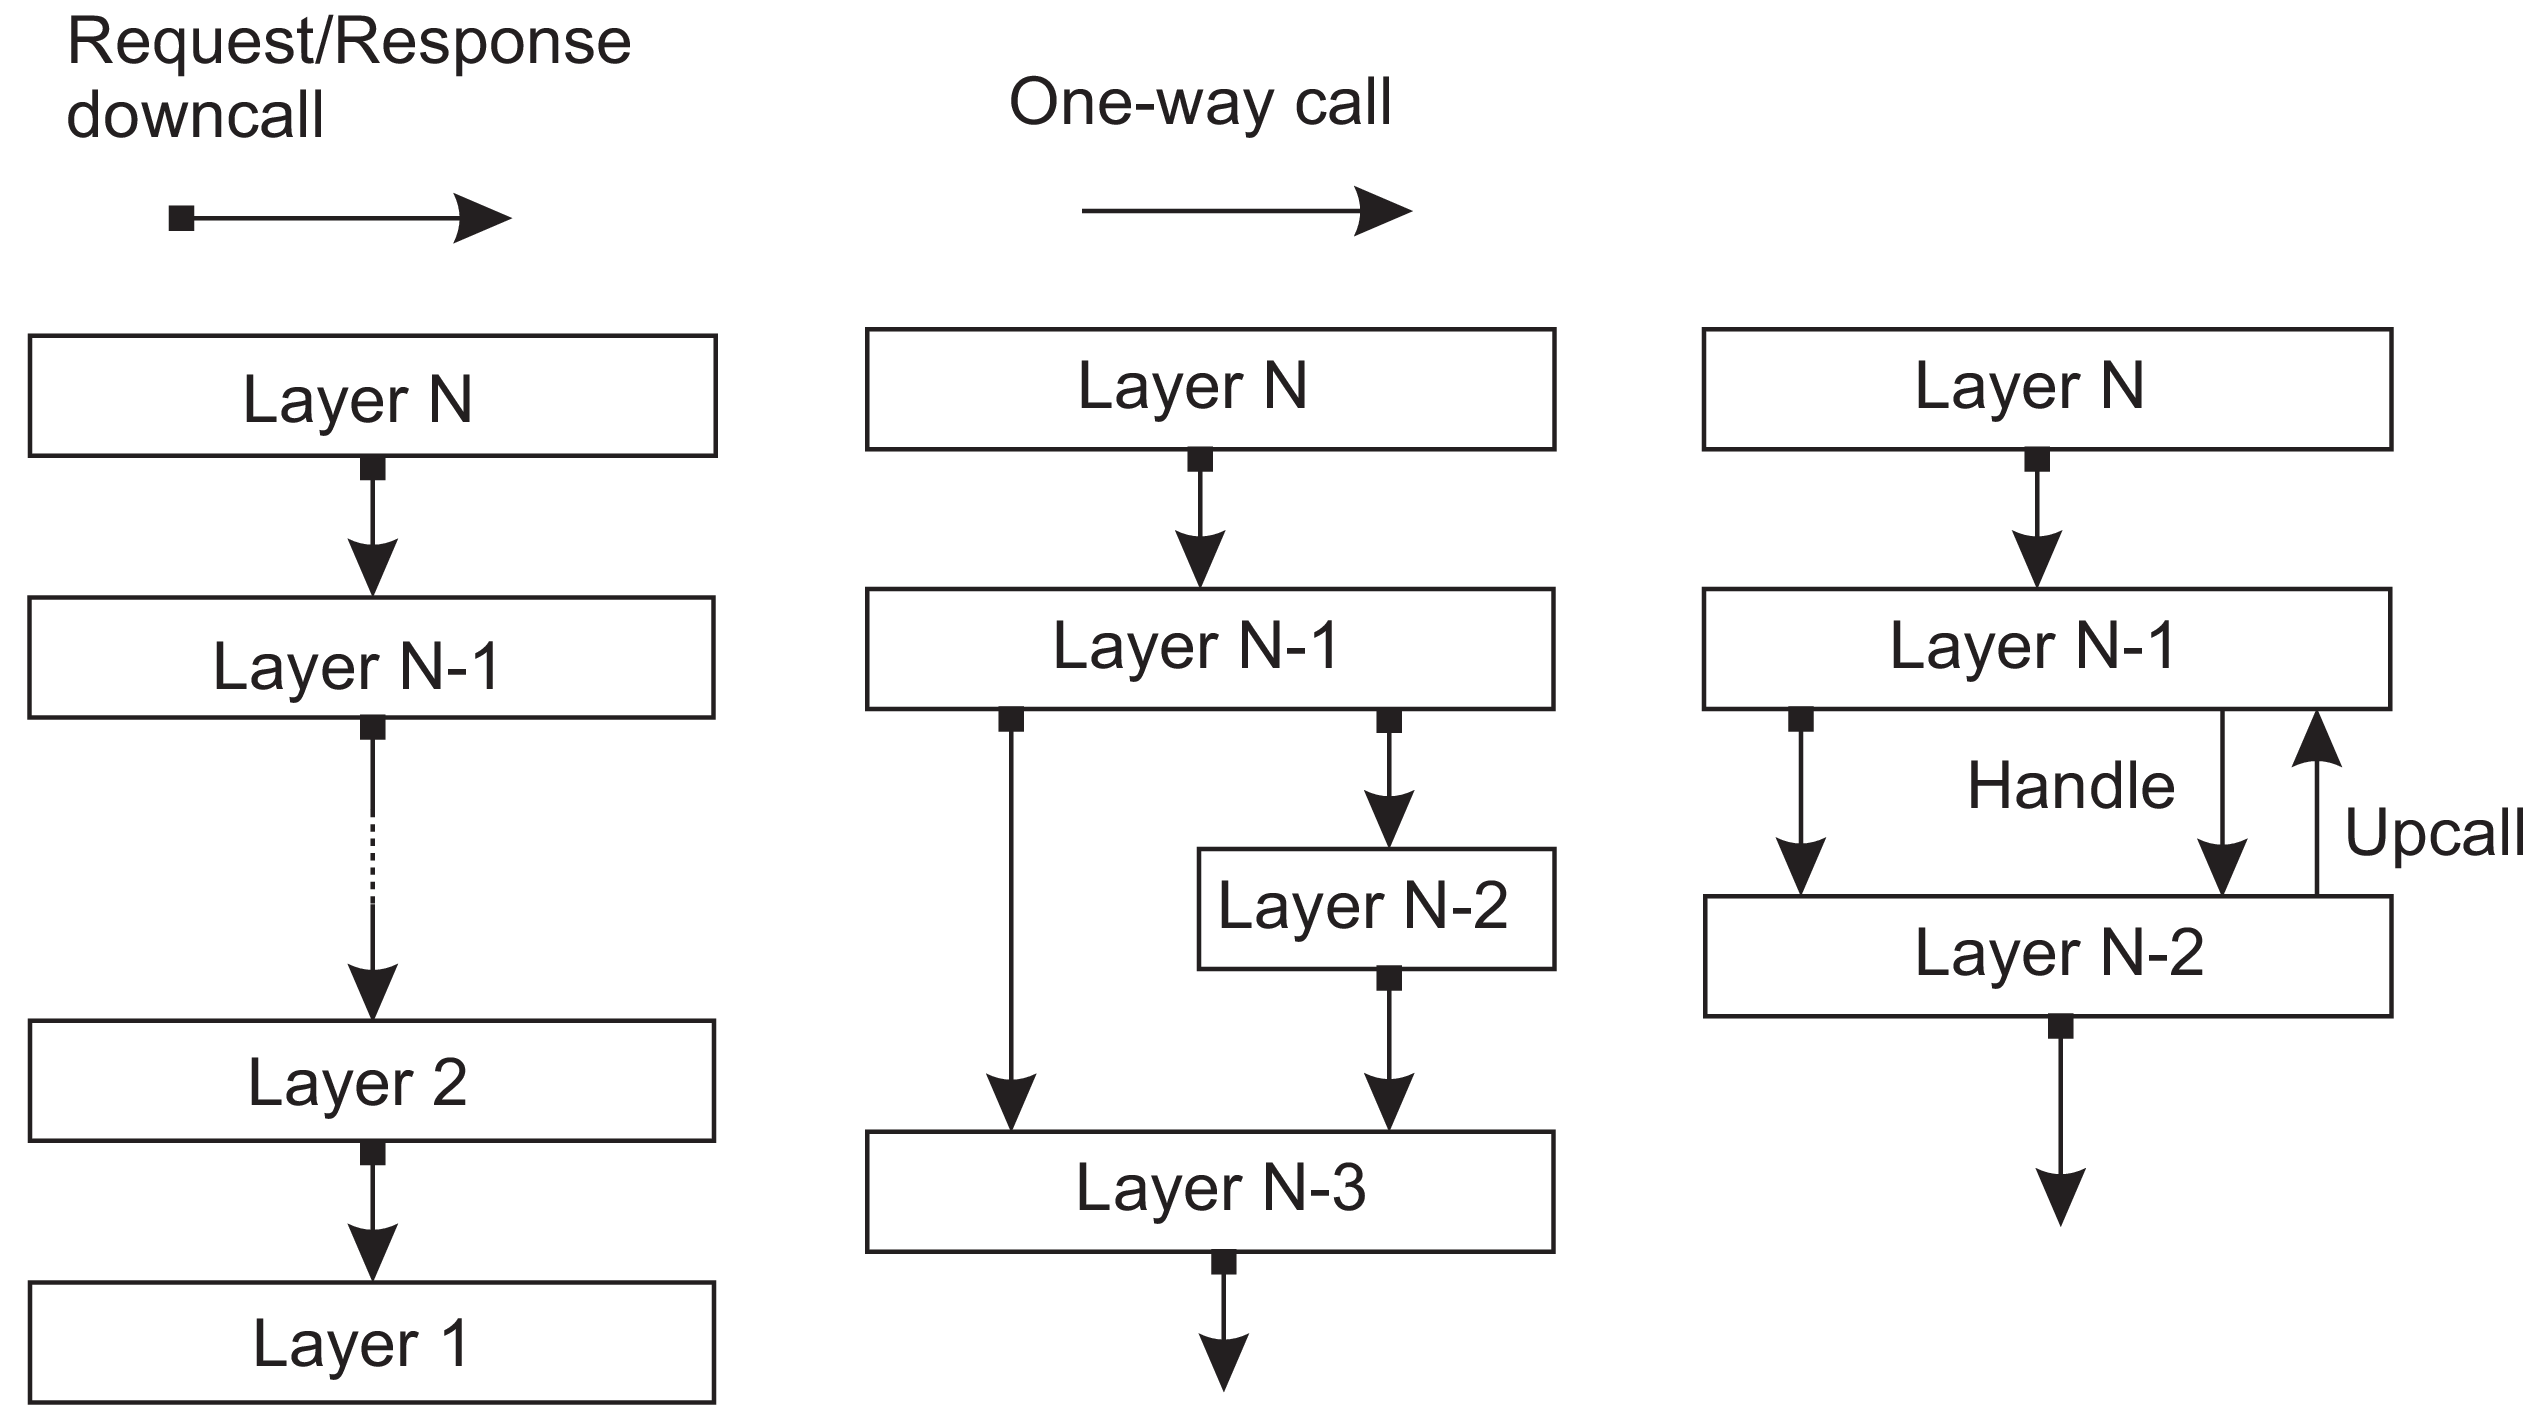
\includegraphics[width=\textwidth]{images/camadas.png}

\end{frame}

%% --------------------------------------------------------

\begin{frame}{Arquiteturas baseadas em camadas - Protocolos}

Uma camada necessriamente tem que se comunicar com outras
\begin{itemize}
    \item A camada deve prover uma interface de comunicação (conector)
    \item Comunicação entre camadas é realizada através deste conector
\end{itemize}

\vspace{0.5cm}

Entretanto, uma camada pode enviar requisições para camadas de outros nós da rede
\begin{itemize}
    \item Tarefa também da interface (conector)
    \item O conector implementa um protocolo de comunicação
    \begin{itemize}
        \item Exemplos de protocolos: TCP e UDP
    \end{itemize}
\end{itemize}
\end{frame}

%% --------------------------------------------------------

\begin{frame}{Arquiteturas baseadas em camadas - Protocolos}

\centering 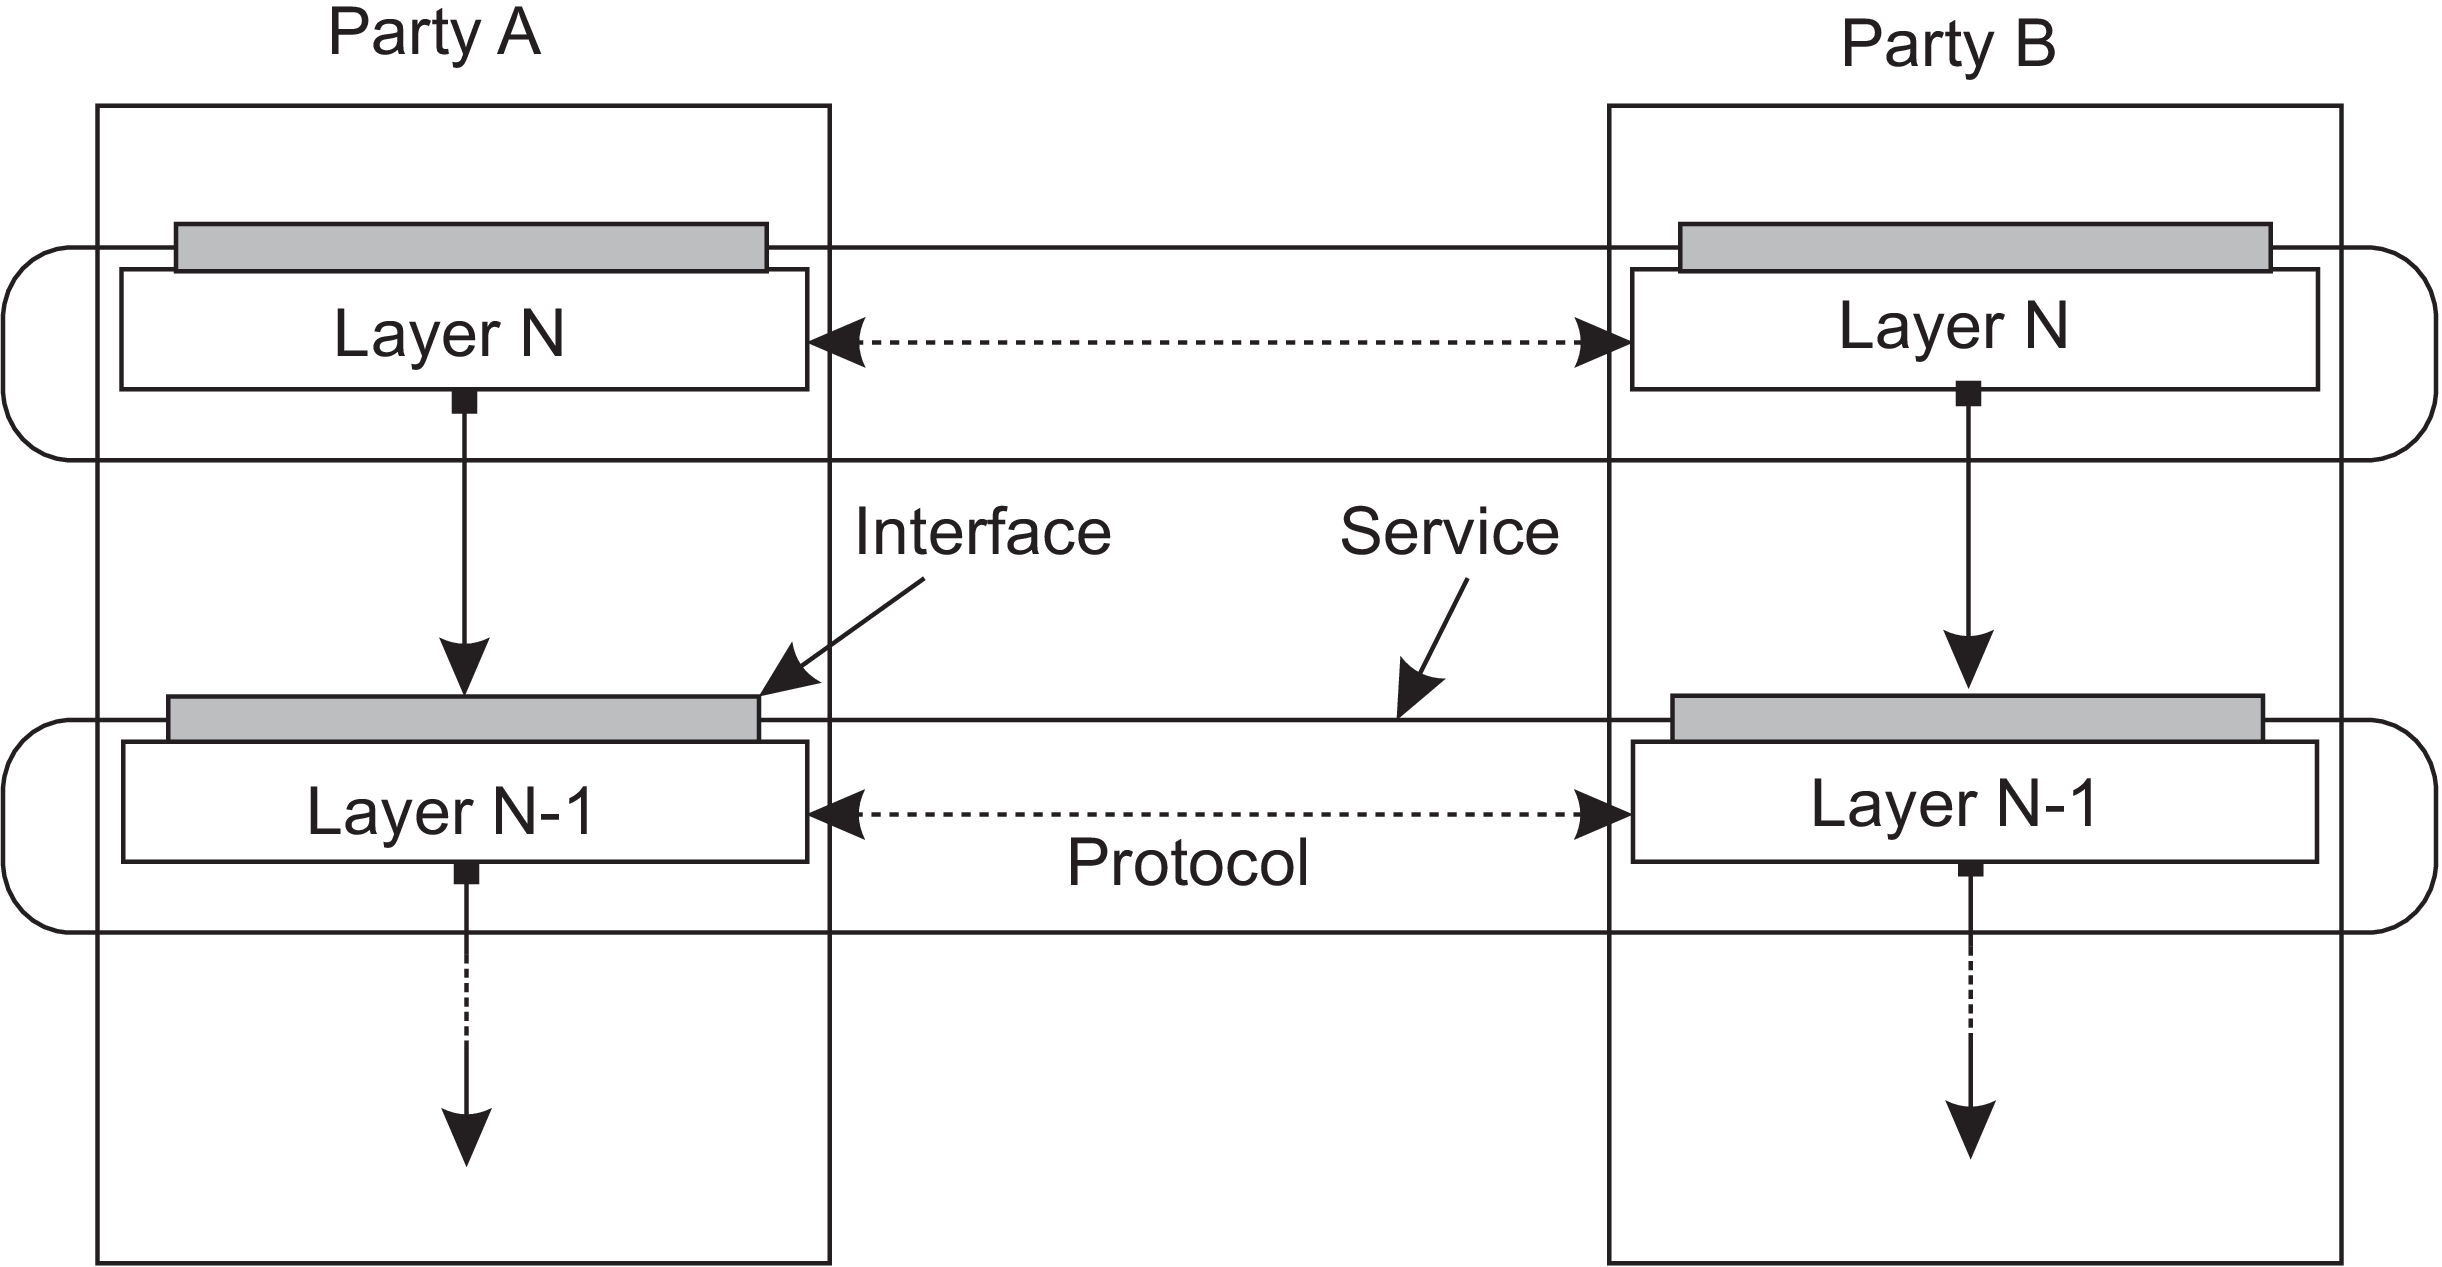
\includegraphics[width=\textwidth]{images/camadas_protocolo.png}
\end{frame}

%% --------------------------------------------------------

\begin{frame}{Exemplo: máquina de busca na web}

\centering 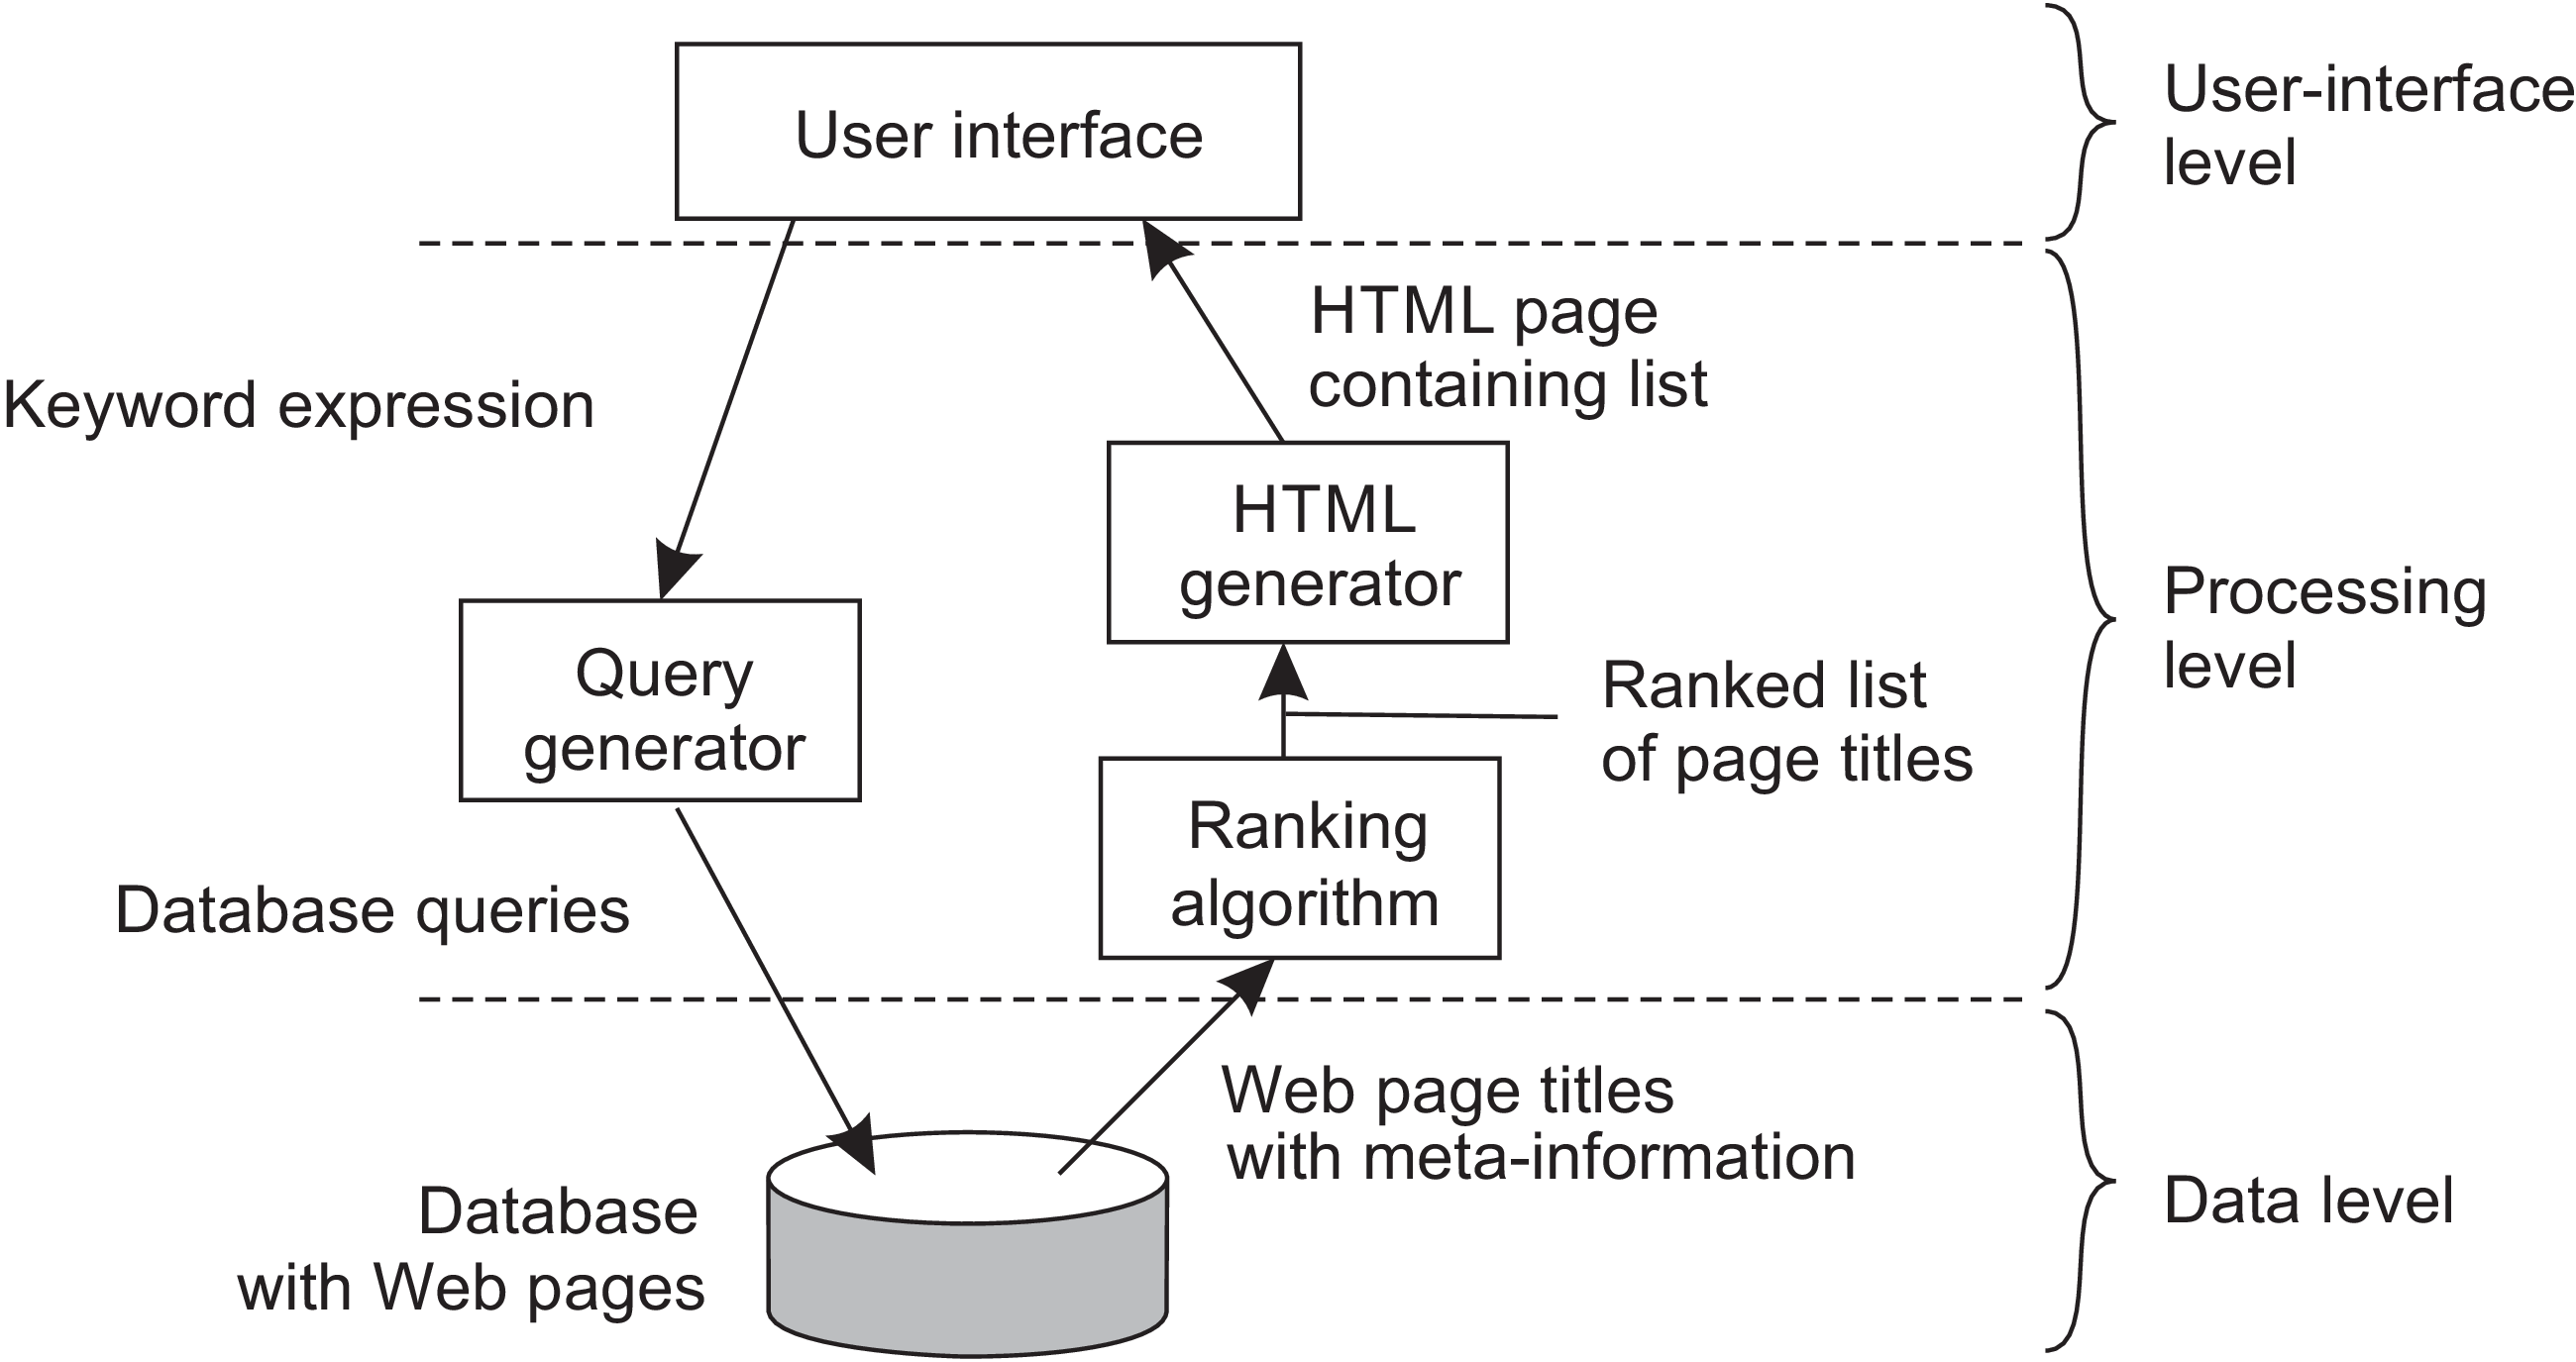
\includegraphics[width=\textwidth]{images/camadas_maquina_busca.png}
\end{frame}

%% --------------------------------------------------------

\begin{frame}{Arquiteturas baseadas em objetos}

Arquitetura de software de um sistema distribuído onde cada componente é um objeto
\begin{itemize}
    \item Extremamente similar ao conceito de orientação de objetos em desenvolvimento de software
\end{itemize}

\vspace{0.5cm}

\centering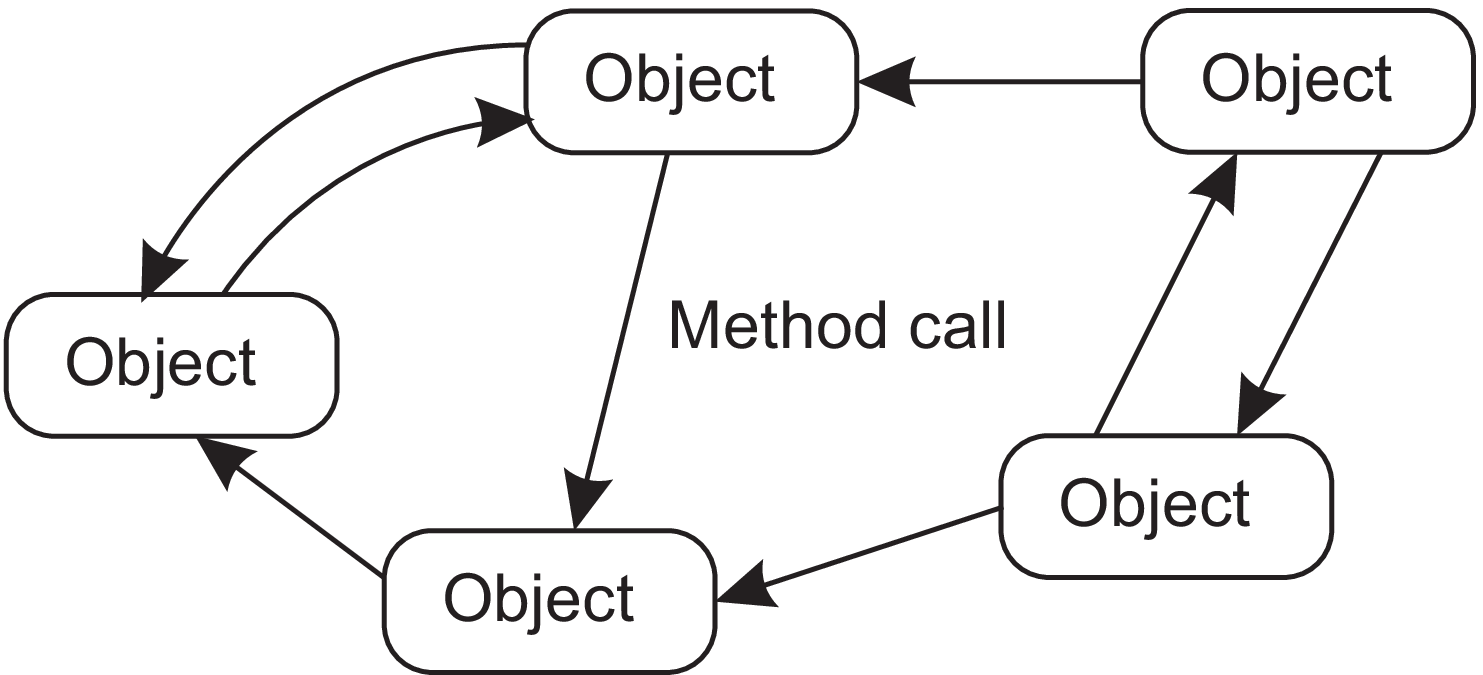
\includegraphics[width=\textwidth]{images/arquitetura_objetos.png}
\end{frame}

%% --------------------------------------------------------

\begin{frame}{Objetos remotos}

É comum que um nó da rede concentre todos os objetos
\begin{itemize}
    \item Somente as interfaces de acesso a eles são disponíveis
    \item Arquitetura orientada a serviços
\end{itemize}

\vspace{0.2cm}

\centering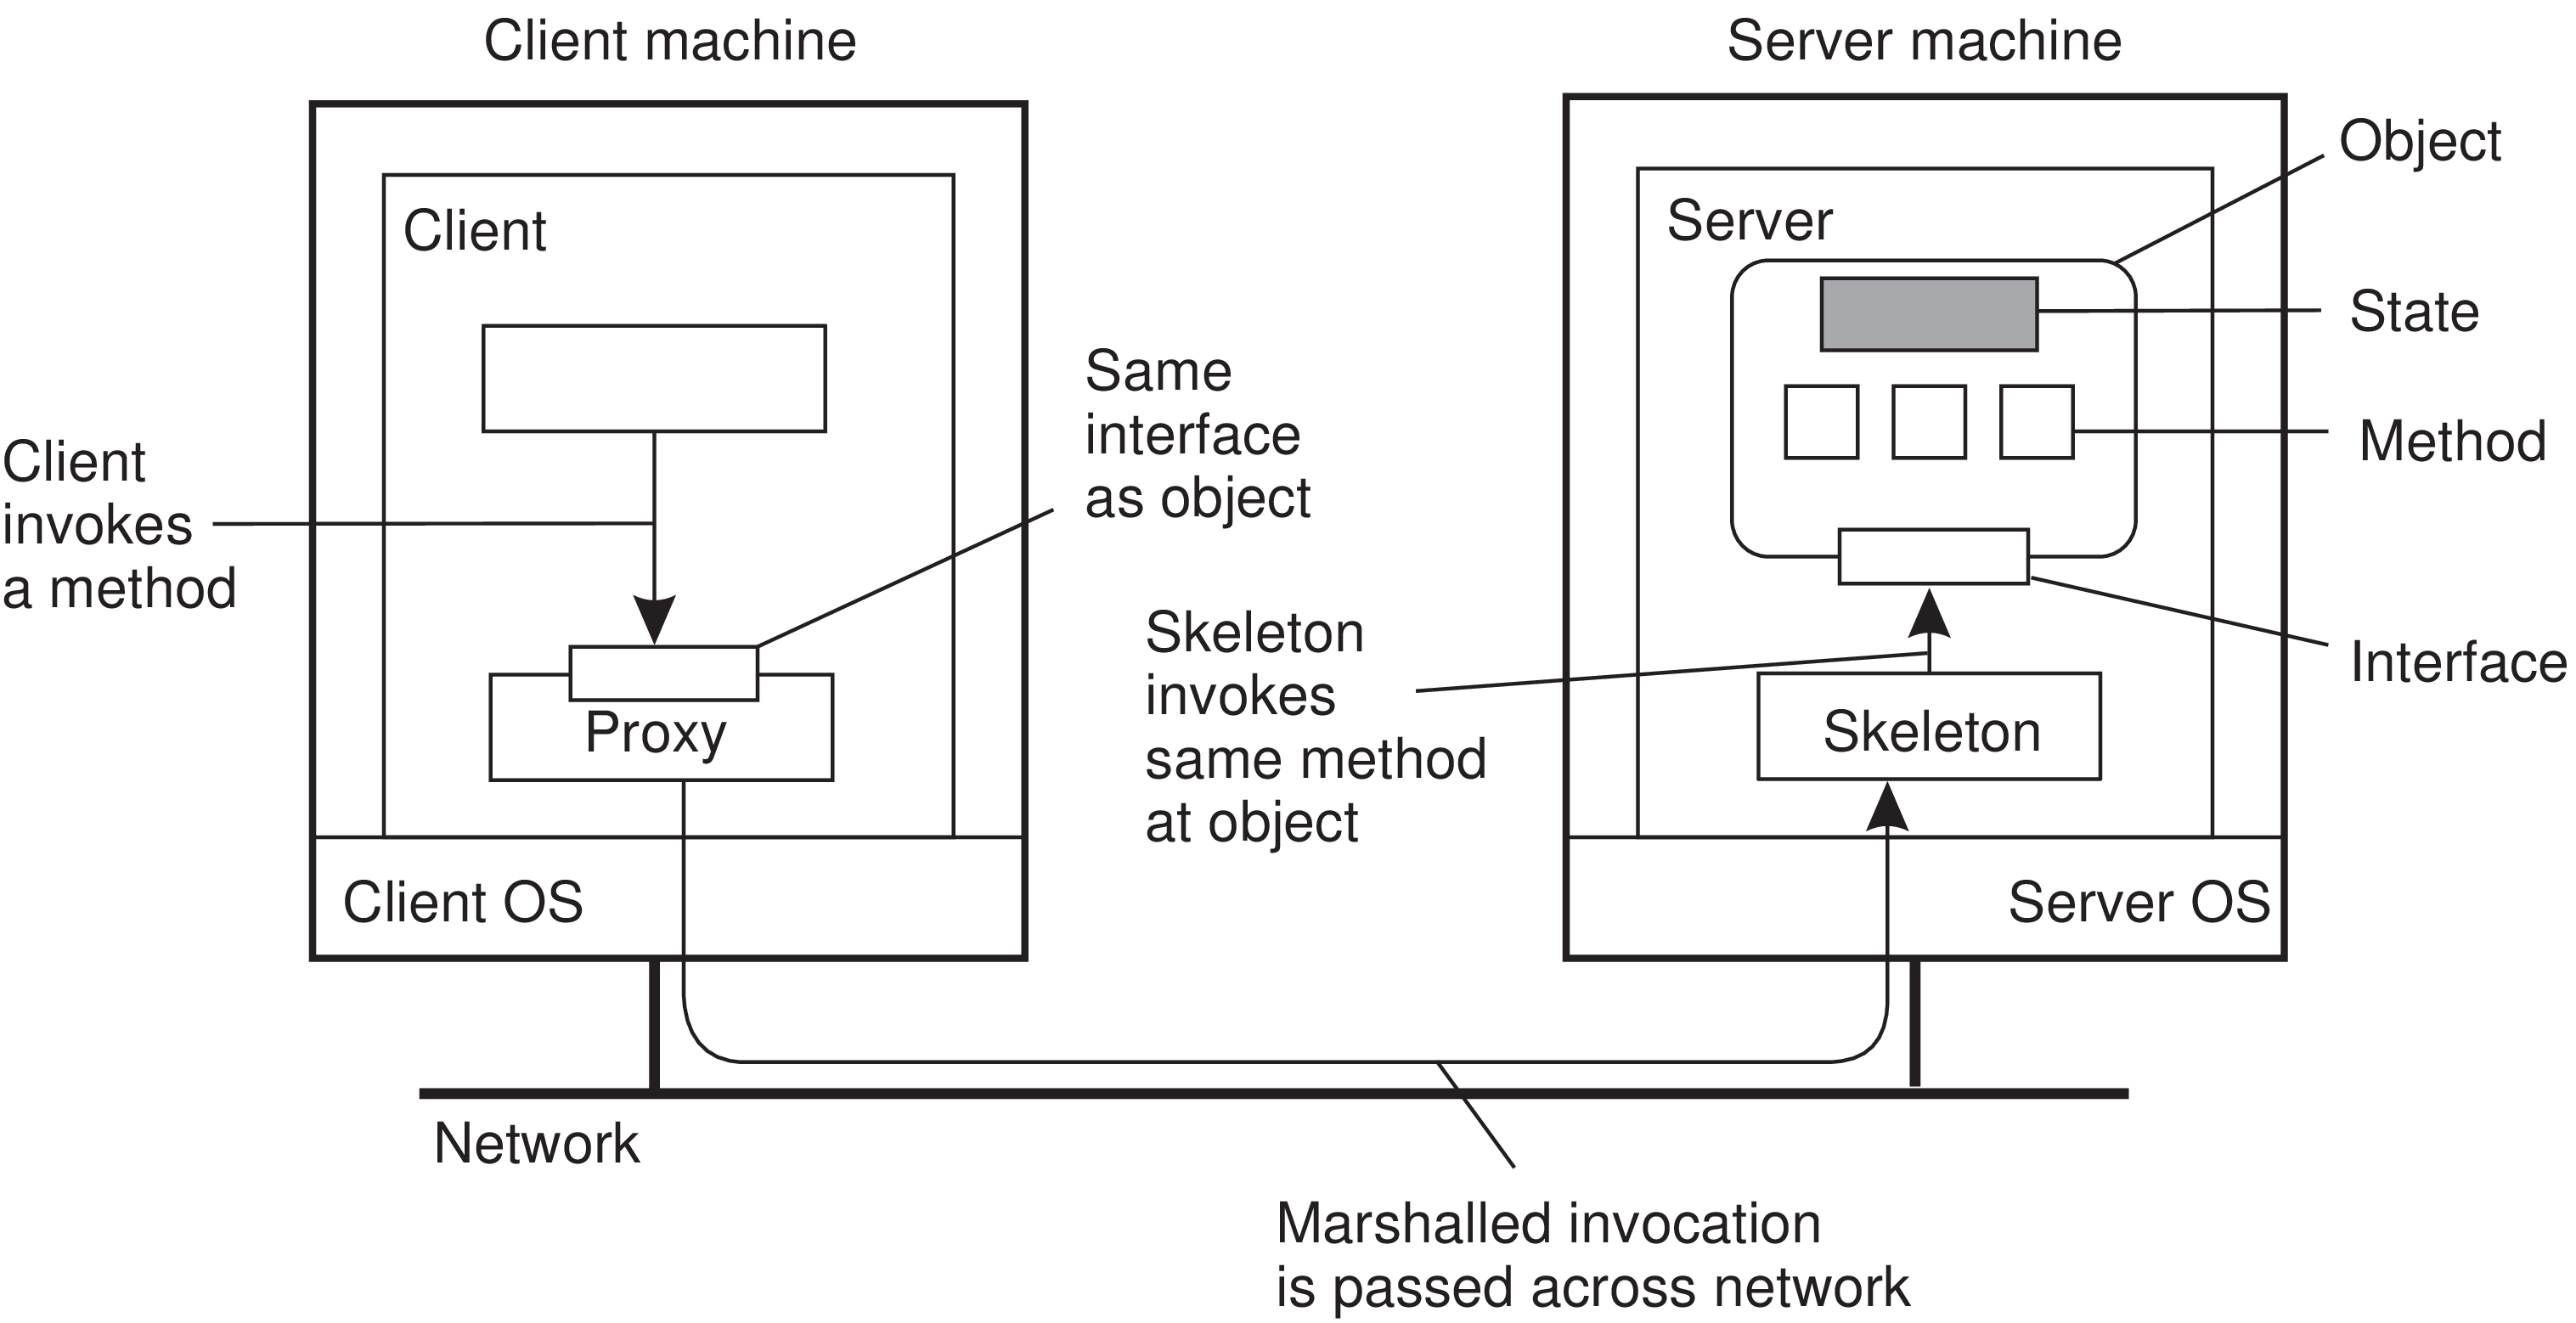
\includegraphics[width=\textwidth]{images/objetos_distribuidos.png}

\end{frame}

%% --------------------------------------------------------

\begin{frame}{Arquiteturas baseadas em recursos}

É uma arquitetura baseada em objetos distribuídos
\begin{itemize}
    \item Serviços REST (Representational State Transfer)
    \item Arquiteturas RESTful
\end{itemize}

\vspace{0.5cm}

É uma maneira ordenada de se implementar diversos objetos distribuídos

\vspace{0.5cm}

Interface oferece quatro operações básicas
\begin{columns}[T]
    \begin{column}{.30\textwidth}
        \begin{itemize}
            \item PUT
            \item GET
        \end{itemize}
    \end{column}
    \begin{column}{.58\textwidth}
        \begin{itemize}
            \item POST
            \item DELETE
        \end{itemize}
    \end{column}
\end{columns}
\end{frame}

%% --------------------------------------------------------

\begin{frame}{Arquiteturas baseadas em eventos}

Também conhecidas como arquiteturas \textit{publish-subscribe}

Neste tipo de arquitetura, existe uma clara separação entre processos e comunicação
\begin{itemize}
    \item Vamos nos focar na coordenação entre processos
\end{itemize}

Comunicação pode ser
\begin{itemize}
    \item Síncrona
    \item Assíncrona
\end{itemize}

Da mesma maneira, podem existir dois tipos de referências na comunicação
\begin{itemize}
    \item Referência explícita
    \item Referência indireta
\end{itemize}
\end{frame}

%% --------------------------------------------------------

\begin{frame}{Arquiteturas baseadas em eventos}

Assim, podemos definir quatro tipos de coordenação de processos, baseados nas diferentes maneiras de referência e comunicação

\begin{table}[]
\def\arraystretch{2.5}
\centering
\resizebox{\textwidth}{!}{%
\begin{tabular}{lccc}
                            & \multicolumn{1}{l}{}           & \multicolumn{2}{c}{Comunicação}                     \\
                            & \multicolumn{1}{c|}{}          & Síncrona           & Assíncrona                     \\ \cline{2-4} 
\multirow{2}{*}{\rotatebox[origin=c]{90}{Referência}} & \multicolumn{1}{c|}{Explícita} & Direta             & Caixa de e-mails               \\
                            & \multicolumn{1}{c|}{Indireta}  & Baseado em eventos & Espaço de dados compartilhados
\end{tabular}%
}
\end{table}

\end{frame}

%% --------------------------------------------------------

\begin{frame}{Direta}

Coordenação direta
\begin{itemize}
    \item Comunicação síncrona
    \item Referência explícita
\end{itemize}

\vspace{0.5cm}

Processos comunicam-se entre si somente se ambos estiverem ativos no mesmo momento

\vspace{0.5cm}

Paralelo com uma ligação telefônica

\end{frame}

%% --------------------------------------------------------

\begin{frame}{Caixa de e-mails}

Coordenação no estilo de caixa de correio (ou e-mail)
\begin{itemize}
    \item Comunicação assíncrona
    \item Referência explícita
\end{itemize}

\vspace{0.5cm}

Processos trocam mensagens entre si
\begin{itemize}
    \item Não precisam estar ativos ao mesmo tempo
    \item Mensagem é enviada e fica aguardando resposta
\end{itemize}

\end{frame}

%% --------------------------------------------------------

\begin{frame}{Espaço de dados compartilhado}

Coordenação no estilo espaço de dados compartilhado
\begin{itemize}
    \item Comunicação assíncrona
    \item Referência indireta
\end{itemize}

\vspace{0.5cm}

\begin{columns}[T]
    \begin{column}{.45\textwidth}
        Um processo envia uma requisição (ou arquivo, ou dado) que fica armazenado em um servidor
        
        \vspace{0.5cm}
        
        Em qualquer momento posterior, outro processo pode acessar o que foi enviado 
    \end{column}
    \begin{column}{.54\textwidth}
        \centering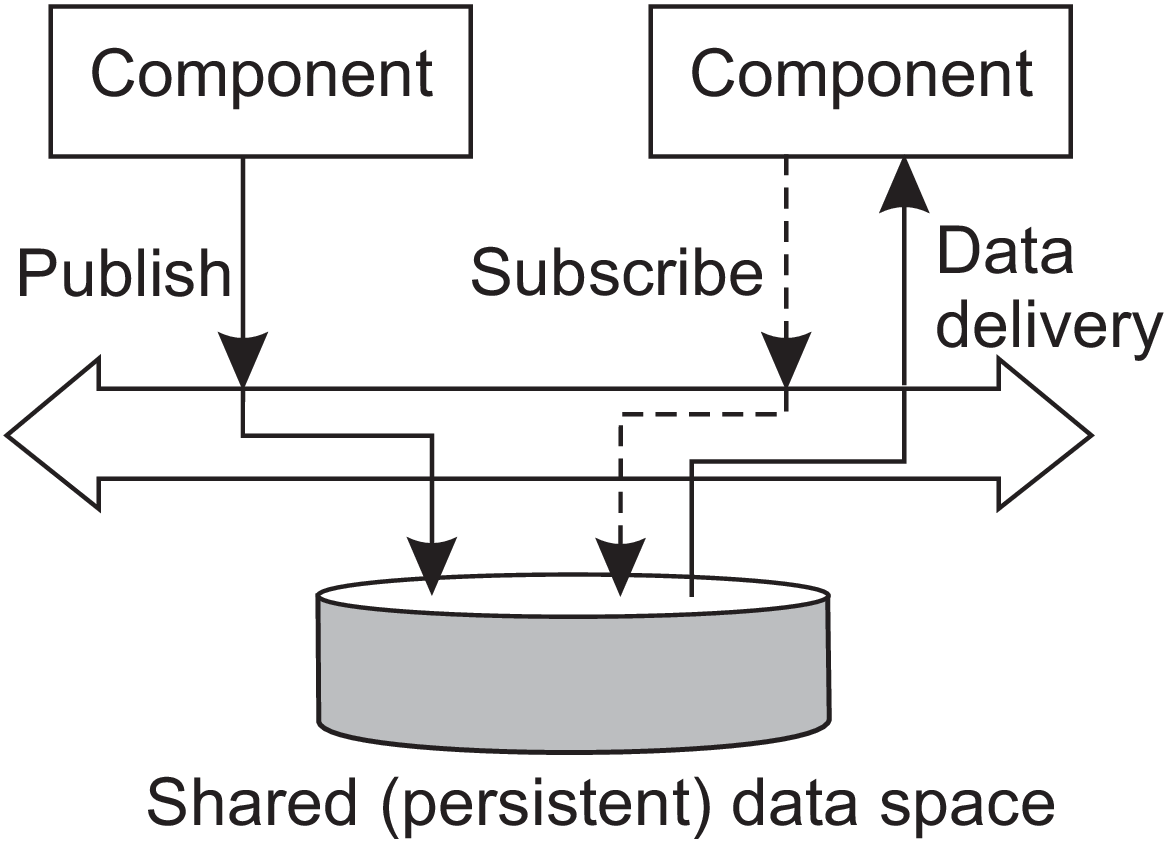
\includegraphics[width=\textwidth]{images/dados_compartilhados.png}
    \end{column}
\end{columns}

\end{frame}

%% --------------------------------------------------------

\begin{frame}{Baseado em eventos}

Coordenação baseada em eventos
\begin{itemize}
    \item Comunicação síncrona
    \item Referência indireta
\end{itemize}

\vspace{0.5cm}

\begin{columns}[T]
    \begin{column}{.45\textwidth}
        Um processo envia uma requisição (ou arquivo, ou dado) 
        
        \vspace{0.5cm}
        
        Cria uma notificação avisando o que ele fez
        
        \vspace{0.5cm}
        
        Outros processos podem acessar
    \end{column}
    \begin{column}{.54\textwidth}
        \vspace{0.78cm}
        \centering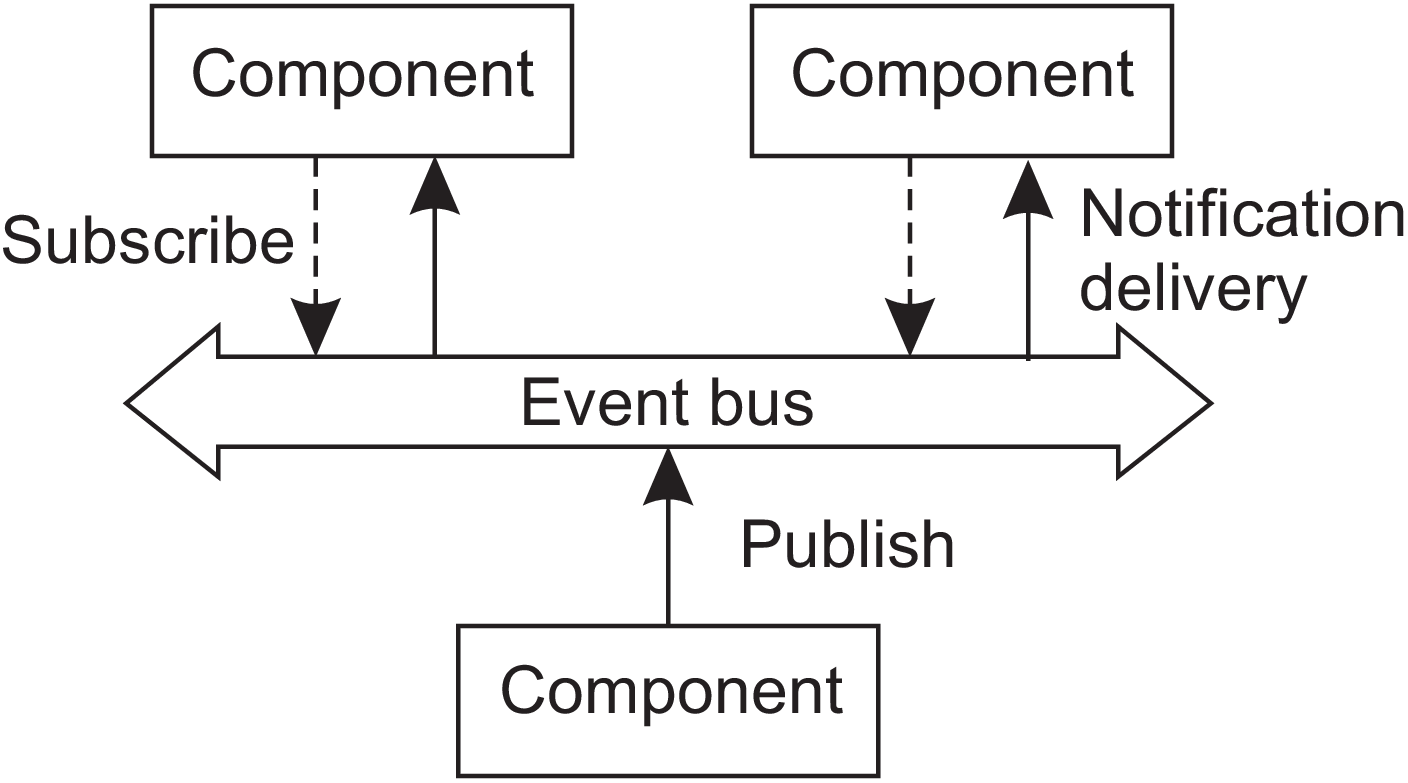
\includegraphics[width=0.95\textwidth]{images/arquitetura_eventos.png}
    \end{column}
\end{columns}

\end{frame}

\begin{frame}{Baseado em eventos}
    
    \vspace{1cm}
    
    \centering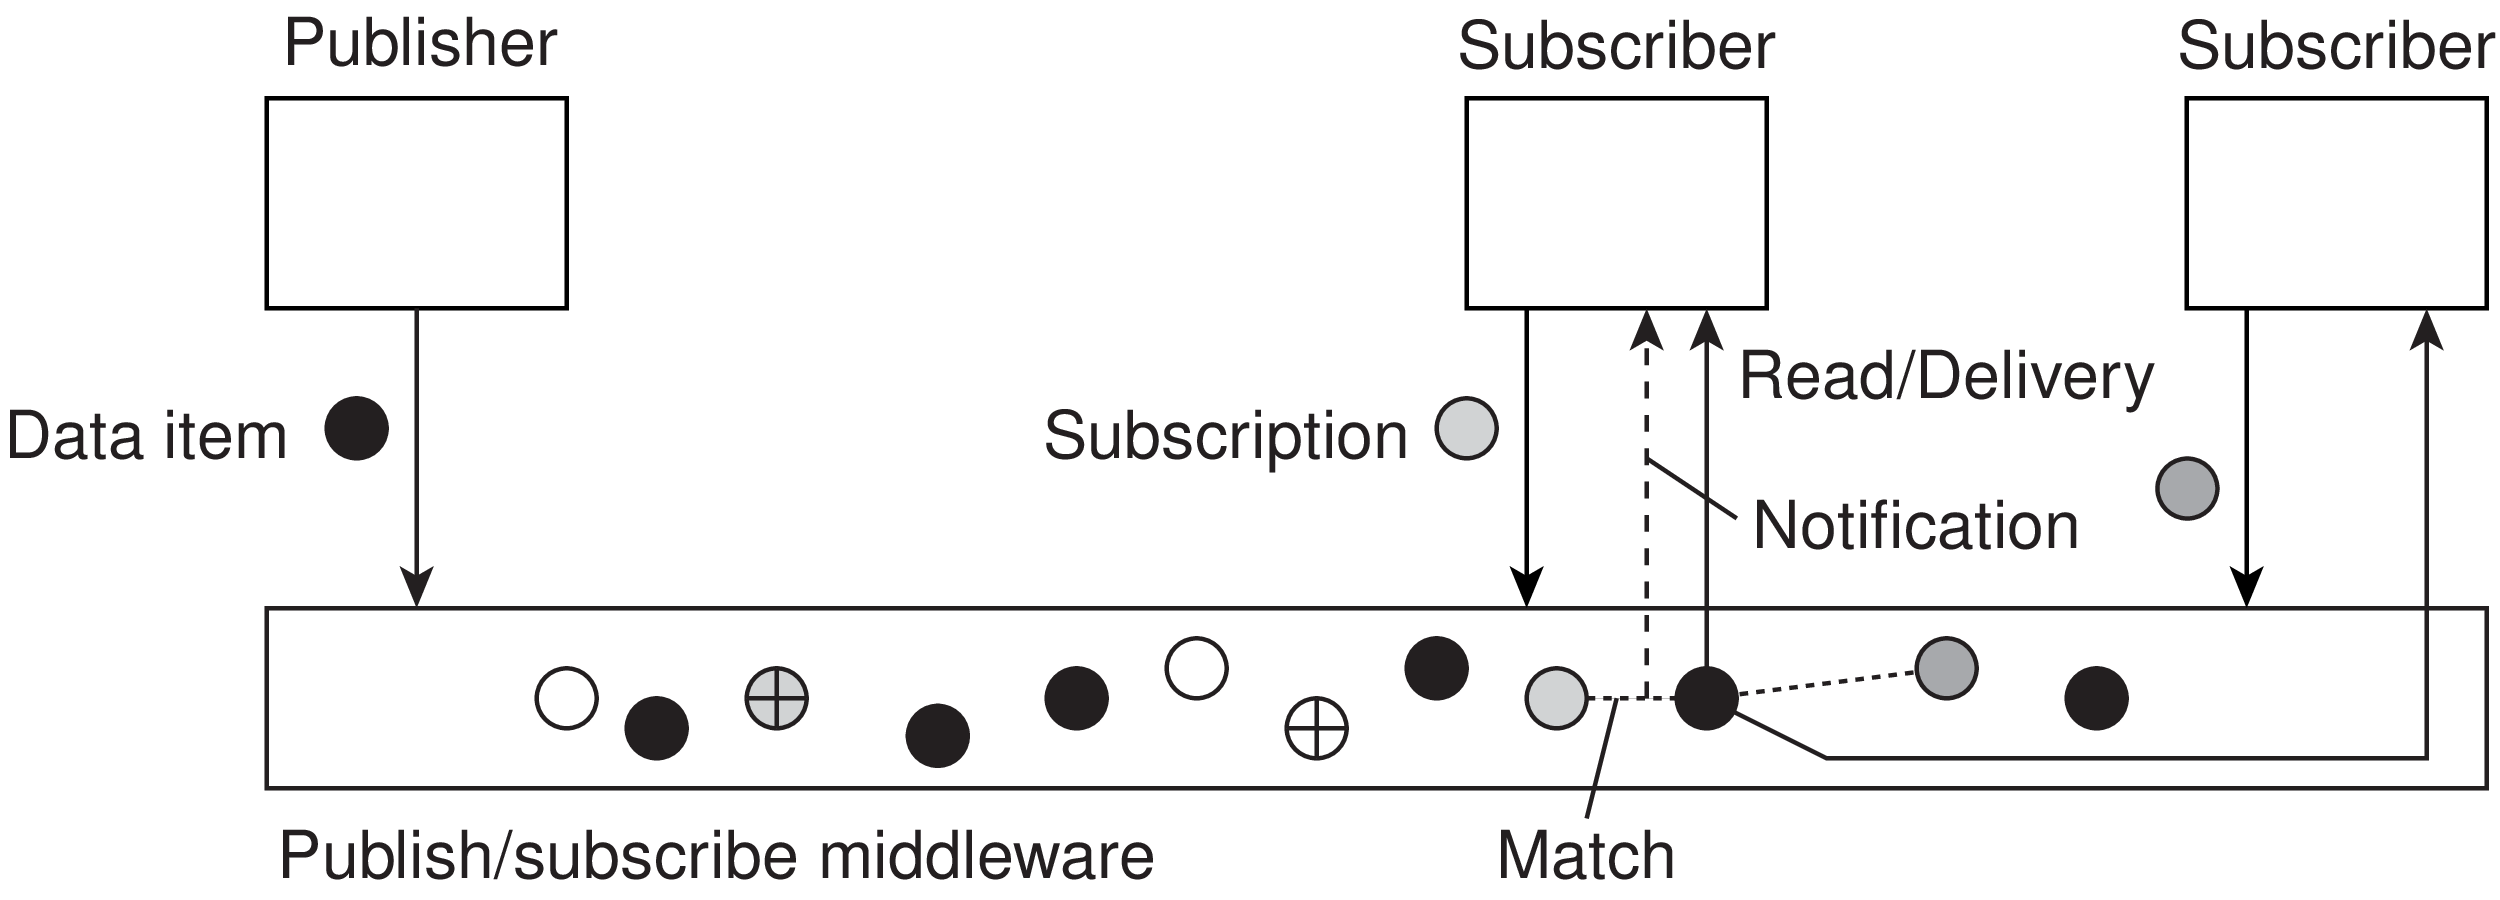
\includegraphics[width=\textwidth]{images/subscribe.png}
    
\end{frame}

\end{document}